%\redpen{
%{\bf  OLD ABSTRACT ---
%  $\eta$~Carinae ($\eta$~Car) is the most massive star
%  known in the Milky Way\cite{DH97}, and a prototype of
%  the poorly understood Luminous Blue Variable stars. 
%  It is in a binary system with a period
%  of 5.52 years\cite{Damineli96}.
%  Since it is one
%  of the few systems close enough (2.3~kpc) to resolve
%  circumstellar material and has evolved on a human timescale, much
%  of our knowledge about the mass loss of massive stars is derived from
%  this system\cite{Smith06}.  It became the second-brightest star in
%  the sky during its mid-19th century ``Great Eruption,'' but then
%  faded from view; only visual estimates of its brightness were
%  recorded and nothing is known about the eruption's spectrum\cite{SF11}.  Here
%  we report the discovery of light echoes of $\eta$~Car which appear
%  to be from the 1838-1858 eruption.  While some of the light from the
%  eruption traveled directly to Earth and was observed in the mid-19th
%  century, light directed away from the Earth scattered off a dust sheet
%  and has now been observed after a half-century delay.  Spectra
%  of these light echoes provide a direct estimate of the effective
%  temperature and other physical properties of this eruption including
%  the expansion speed, 
%  raising questions about traditional scenarios for the eruption that
%  involve a minimum temperature for steady opaque winds.
  %raising questions about traditional scenarios for the outburst that involve opaque winds.  
%  We also find important
%  differences between the light-echo spectra of $\eta$~Car and spectra
%  of extragalactic transients previously presumed to be analogues.
%}
%}

%\bluepen{
%Eta Carina is a massive binary system (period of 5.52 years\cite{Damineli96}) at a
%distance of 2.3 kpc. It underwent a 'great eruption' with three
%optical peaks\cite{SF11} in 1838, 1843 and 1845 during which it is
%believed to have ejected more than 10~$M_{\odot}$, releasing
%\about10\% of the energy of a core-collapse
%supernova\cite{Smith03,Smith08}, although the star survived the
%event. Studies of transient events in other galaxies suggest that the
%mechanism could be explosions or extreme winds\cite{Smith11}, but
%their diversity leads to uncertainty about which model explains
%$\eta$~Car. Here we report observations of light echoes from
%(probably) the 1843 event that reveal that the expectations of an
%opaque-wind model\cite{Davidson87} are inconsistent with the outburst
%spectral type (G2-G5) and lack of \ion{Ca}{II} emission. From the
%data, we conclude that a hydrodynamic explosion
%mechanism\cite{Damineli96,Smith03,Smith08} must be responsible for the
%dramatic brightenings of $\eta$~Car. Compared to other extragalactic
%transients, $\eta$~Car is more extreme in terms of radiated energy
%(10$^{49.3}$~erg), kinetic energy ($>$$10^{50}$~erg) and duration
%(decades).
%}

{\bf 
$\eta$~Carinae is one of the most massive binary stars  in the
Milky Way\cite{DH97,Damineli96}. It became the second-brightest star
in the sky during its mid-19th century ``Great Eruption,'' but then
faded from view (with only
naked-eye estimates of brightness\cite{Frew04,SF11}).
%No contemporaneous spectroscopy of the Great Eruption
%exists - only visual brightness estimates\cite{Frew04,SF11}.
%No measurements of the Great Eruption with modern instrumentation exist - 
%only by-eye brightness estimates\cite{Frew04,SF11}.
Its eruption is unique among known astronomical transients in that it
exceeded the Eddington luminosity limit for 10 years.
%\redpen{maintained a high outburst luminosity (bolometric magnitude of -14)
%for 10 years.}
Because it is only 2.3~kpc away, spatially resolved studies of the
nebula have constrained the ejected mass and velocity, indicating that
in its 19th century eruption, $\eta$~Car ejected more than
10~$M_{\odot}$ in an event that had 10\% of the energy of a typical
core-collapse supernova\cite{Smith03,Smith08} without destroying the
star.
%\redpen{Because it is in our Galaxy, spatially resolved studies
%of the nebula have been able to show that it ejected more than
%10~$M_{\odot}$, 1-2 orders of magnitude more than other known
%outbursts of this type, and releasing \about10\% of the energy of a
%core-collapse supernova \cite{Smith03,Smith08} without destroying the
%star.}
%Until now, the lack of spectra has limited our ability to determine
%what physical mechanisms caused this eruption.
%
Here we report the discovery of light echoes of $\eta$~Carinae which
appear to be from the 1838-1858 Great Eruption.  
Spectra of these light echoes show only absorption lines, which are
blueshifted by $-$210~km~s$^{-1}$, in good agreement with predicted
expansion speeds\cite{Smith08}.
%at lower latitudes. 
The light-echo spectra correlate best with those of G2-G5 supergiant
spectra, which have effective temperatures of $\sim$5000~K.  In
contrast to the class of extragalactic outbursts assumed to be analogs
of eta Carinae's Great
Eruption\cite{Goodrich89,Humphreys94,Humphreys99,VanDyk00,Vink09,Kashi10_ngc300},
the effective temperature of its outburst is significantly cooler than
allowed by standard opaque wind models\cite{Davidson87}.  This
indicates that other physical mechanisms like an energetic blast wave
may have triggered and influenced the eruption.
}

\medskip

%\section{Introduction}

%%Light echoes arise when light from luminous astrophysical transients
%%scatters off interstellar dust. Due to the longer path length, the
%%echoes reach the Earth later than the light arriving
%%directly\cite{Kapteyn02,Couderc39}.  These echoes afford unique
%%opportunities to study light from historical outbursts using modern
%%instruments\cite{Rest05b,Rest08a}.

%Because of its proximity, $\eta$~Carinae ($\eta$~Car) is probably the
%most intensely scrutinized massive star system. It lies at the heart
%of the Carina star-forming region, is surrounded by an intricate
%circumstellar nebula ejected during the Great Eruption, has
%spectacular variability at all wavelengths\cite{DH97}, and is in a
%binary system with a period of 5.52 years\cite{Damineli96}.

%%\redpen{Remove, or sub with a summary? The Great Eruption is thought to have
%%ejected more than 10~$M_{\odot}$ from the star, and to have released
%%about 10\% of the energy of a core-collapse supernova
%%(SN)\cite{Smith03,Smith08}, even though the star survived the event.
%%The underlying physical mechanism of the outburst remains
%%unexplained.}  

%Some extragalactic non-SN transients have been
%interpreted as analogues of the Great Eruption of $\eta$~Car
%\cite{Goodrich89,Humphreys94,Humphreys99,VanDyk00,Vink09,Kashi10_ngc300}. 
%However, their widening diversity calls into question their
%association or suggests that massive eruptions like $\eta$~Car are
%only a subset of non-terminal
%eruptions\cite{Smith11}. 

%%\bluepen{Comparisons between $\eta$~Car and
%%its extragalactic analogues have been limited by the lack of spectra
%%of the eruption itself.}
%%\redpen{An important
%%gap in our understanding is that until now we have had only visual
%%brightness estimates for the Great Eruption of $\eta$~Car\cite{SF11},
%%whereas we have modern spectra and precise photometry for the
%%extragalactic transients.}
%\bluepen{An important
%gap in our understanding is that until now the comparison between $\eta$~Car and
%its extragalactic analogues has been strongly limited by the lack of spectra
%of the Great Eruption, whereas we have modern spectra and precise photometry for the
%extragalactic transients.}



$\eta$~Car-like giant eruptions of Luminous Blue Variables (LBVs) are
characterized by significant mass-loss and an increase in luminosity
by several magnitudes\cite{Humphreys94,Humphreys99}.
%$\eta$~Car-like giant eruptions are characterized by visual brightness
%of greater than 3 magnitudes, an increase in the bolometric
%luminosity, and an increase in the mass-loss
%rate\cite{Humphreys94,Humphreys99}.  
Traditionally, it was thought
that this increase in luminosity 
drives a dense wind, producing an
optically-thick cooler pseudo-photosphere with a minimum effective
temperature of ~7000 K and an F-type spectrum\cite{Davidson87}.  Within
this model, $\eta$~Car has been considered the prototype of the
so-called ``supernova imposters''
\cite{Goodrich89,Humphreys94,Humphreys99,VanDyk00,Vink09,Kashi10_ngc300}.

%Some extragalactic non-SN transients have been
%interpreted as analogues of the Great Eruption of $\eta$~Car
%\cite{Goodrich89,Humphreys94,Humphreys99,VanDyk00,Vink09,Kashi10_ngc300}. 
%However, their widening diversity calls into question their
%association or suggests that massive eruptions like $\eta$~Car are
%only a subset of non-terminal
%eruptions\cite{Smith11}. 


% at least several times
%the original radius.  This model predicts a minimum effective
%temperature of ~7000 K (and F-type spectrum), arising from the
%temperature dependence of the wind opacity\cite{Davidson87}.  

We obtained images in proximity to $\eta$~Car
(Figure~\ref{fig:diffim}) that, when differenced, show a rich set of
light echoes. The largest interval between our images is 8 years.  We
have also found similar echo candidates at other positions, which we
are currently monitoring.  The large brightening and long duration
point to the Great Eruption as the source of the light echoes.  We
have also obtained a composite light curve in the SDSS $i$ filter of
the light echoes (see Fig.~\ref{fig:lc}),
showing a slow decline of several tenths of a magnitude over half a
year.  This light curve is most consistent with the historical
observations\cite{SF11} of a peak in 1843, part of the 1838-1858 Great
Eruption, although further observations are necessary to be certain
(see the Supplementary Information, SI).

%\begin{figure}%[t]
%  \caption{
%\ifastroph
%    
\includegraphics[scale=0.97]{diffimfigure/etacar_diffim_slit.jpg}
%\else
%  \ifsuppl
%    
\includegraphics[scale=0.97]{diffimfigure/etacar_diffim_slit.jpg}
%  \fi
%\fi
%$\eta$~Car light echoes. The left panel shows the positions of
%$\eta$~Car and our images (white box), plotted on an image
%in the light of 3 different emission lines:
%oxygen (blue), hydrogen (green), and sulfur (red) (credit:
%Nathan Smith, University of Arizona/NOAO/AURA/NSF).
%The middle panels show the images obtained with the CTIO 4-m
%Blanco telescope of a region $\sim$0.5~degrees to the south of
%$\eta$~Car at epochs 2003 March 10 ({\it A}), 2010 May 10 ({\it B}),
%and 2011 Feb 6 ({\it C}), from top to bottom.  The right panels show
%the difference images {\it C-A} and {\it C-B} at the top and middle,
%respectively. Example light-echo positions are indicated with blue
%(epoch {\it A}) and red (epoch {\it B} and {\it C}) arrows.  The
%bottom right panel shows a zoom of the spectrograph slit, indicated
%with a blue line.  For all panels north is up and east is to the left.
%Applying the vector method that previously allowed us to identify the
%source of the light echoes from the supernovae (SNe) that produced the
%SN remnants 0509$-$67.5, Cas~A, and Tycho\cite{Rest05b,Rest08b}, we
%find that a dramatic brightening of $\eta$~Car must be the origin.  In
%these echoes, unlike those of Galactic SNe\cite{Rest11_leprofile},
%there is still significant spatial overlap even at separations of one
%light-year, suggesting that the duration of the event causing them
%must be significantly longer than one year.  We also see brightening
%of 2 magnitudes or more within 8 years.  Thus, the Lesser Eruption
%from 1887 to 1896, which brightened by only a magnitude, is excluded
%as the source.
%\label{fig:diffim}}
%\end{figure}

%\begin{figure}
%\caption{
%%\ifastroph
%  
\includegraphics[scale=1.05]{lc/lc_noblkline.jpg}
%\else
%  \ifsuppl
%    
\includegraphics[scale=1.05]{lc/lc_noblkline.jpg}
%  \fi
%\fi
%Historical and light-echo lightcurve of $\eta$~Car. The historical
%light curve\cite{SF11} in visual apparent magnitudes is shown with
%black circles and lines, with error bars indicating approximate
%uncertainties in these eye estimates.  Light echo brightnesses (SDSS
%$i$; error bars are the s.d.) from our eight modern images spanning
%$\sim$8~years are displayed shifted by 174.2~yrs (green circles),
%167.95~yrs (red circles), and 166.28~yrs (blue circles), in order to
%illustrate the best-matching time delays for the 1838, 1843, and 1845
%outbursts, respectively.
%The first epoch is an upper limit indicated with an arrow. 
%The upper panel shows the full time range of the Great
%Eruption and therefore shows all three potential matches, whereas the
%lower panels show the brightnesses from seven of our eight modern
%epochs in a magnified time period around each peak.
%\label{fig:lc}}
%\end{figure}

Spectra of the light echoes (see Figure~\ref{fig:spec}) show
only absorption lines characteristic of cool stellar photospheres, but
no evidence of emission lines.  In 
particular the
\ion{Ca}{II} infrared (IR) triplet is only in absorption.
%Three spectra of the light echo are shown in Figure~\ref{fig:spec} ---
%the positions differ only slightly in slit angle (see Table~S1).
%The light-echo spectra show only absorption lines characteristic of
%cool stellar photospheres, but no evidence of emission lines.  In
%particular the
%\ion{Ca}{II} infrared (IR) triplet is only in absorption.
%The right panel of Figure~\ref{fig:spec} shows the region of H$\alpha$
%and [\ion{N}{II}]. 
Because of bright ambient nebular emission, it is
difficult to determine if there is any H$\alpha$ emission from $\eta$~Car
itself, but in any case it must be weak if present.  By
cross-correlating each of our $\eta$~Car echo spectra with the UVES
spectral library\cite{Bagnulo03} (see
Figure~S2~and~S3) 
\ifcheck
  \redpen{CHECK S\ref{fig:speclines}~and~S\ref{fig:pdf}}
\fi
we find best agreement
with supergiant spectral types in the range of G2-G5, with an
effective temperature of $\sim$5000~K. Spectral types of F7 or earlier
are ruled out by our analysis (see SI for more details).

%The
%reason is that regions with scattering dust have different densities
%of hydrogen than regions without. Therefore we can expect to have
%background emission lines with different strengths at the position
%where the light echo is compared to the position without light echoes
%that is used for determining the background.

%Similarly to some other LBV-like eruptions, the light-echo spectra shown in the
%left panel of Figure~\ref{fig:spec} are dominated by absorption lines
%characteristic of cool stellar photospheres. In particular, the
%\ion{Ca}{II} IR triplet is in absorption and not in emission. The
%right panel of Figure~\ref{fig:spec} shows the H$\alpha$ and
%[\ion{N}{II}] lines. Subtracting the H II region emission lines has
%proven to be difficult and inaccurate. The reason is that regions with
%scattering dust have different densities of hydrogen than regions
%without. Therefore we can expect to have background emission lines
%with different strengths at the position where the light echo is
%compared to the position without light echoes that is used for
%determining the background.

%
%\begin{figure}
%\caption{
%\ifastroph
%  
\includegraphics[scale=0.57]{specfigure/eta03_spec.pdf}
%\else
%  \ifsuppl
%  
\includegraphics[scale=0.55]{specfigure/eta03_spec.pdf}
%  \fi
%\fi
%Light echo spectra of $\eta$~Car's Great Eruption.  The three optical
%low-resolution spectra of the light echo (black lines) were taken at
%J2000 position RA=10:44:12.127 and Decl.=$-$60:16:01.69 in March and
%April 2011 obtained at the Magellan~I 6.5-m and du~Pont 2.5-m
%telescopes of the Las Campanas Observatory, Chile. 
%A log of the spectroscopic observations and
%details of the spectra is presented in Table~S1.
%\ifcheck
%  \redpen{CHECK} 
%\fi
%The slit positions differ only slightly in slit angle.
%The spectra were reduced using standard techniques and then
%wavelength-calibrated using observations of an HeNeAr lamp. The
%wavelength calibration was checked and corrected using night-sky
%emission lines, especially \ion{O}{I} 5577\AA, and OH lines in the red
%part of the spectrum. We flux-calibrated the spectra using a flux
%standard observed the same night as the science observations.  The
%%left panel shows the spectra from 5000 to 9000\AA.  The spectra are
%not corrected for reddening nor for the blue-ward scattering by the
%dust.  The blue lines show for comparison spectra of three examples of
%SN imposters: SN~1997bs, SN~2009ip, and UGC~2773-OT1.  The right panel
%shows the H$\alpha$ and [\ion{N}{II}] emission lines. Note that the
%background emission-line subtraction is incomplete since they
%spatially vary. Also, for
%%\specMhi\ H$\alpha$ is at the edge of the chip and is therefore uncertain.
%\label{fig:spec}}
%%\end{figure}


%This relatively cool apparent temperature derived from the spectral
%type is in accord with the reddish or ``ruddy'' colour noted by visual
%observers during the Great Eruption\cite{SF11}.  The temperature
%inferred from the spectral type is, however, much more reliable than
%an apparent colour since it is not influenced by reddening due to
%unknown amounts of new dust formation along the sightline.

% or
%contamination by very strong line emission, both of which are likely
%to be present in $\eta$ Car's eruption.

%\subsection{Velocity and Asymmetry of the \ion{Ca}{II} IR triplet}

Doppler shifts of absorption features in the echo spectra provide direct
information about the outflow speeds during the eruption.
The \ion{Ca}{II} IR triplet absorption features in the spectrum are
noticeably blueshifted (see Figure~S2).
\ifcheck
  \redpen{CHECK S\ref{fig:speclines}}
\fi
By cross-correlation with G-type\cite{Cenarro01} templates, we determine
velocities of $-202\pm9$, $-210\pm14$, and $-237\pm17$~km~s$^{-1}$ for
our three individual spectra and an average
velocity of $-210\pm30$~km~s$^{-1}$, which includes an uncertainty for
the dust sheet velocity.



The bipolar nature of the Homunculus shows that the $\eta$~Car
Great Eruption was strongly aspherical.  It was previously predicted
that the outflow speeds one would derive from spectra of $\eta$~Car in
outburst, looking at the poles and equator of the double lobes, would
be $\sim-$650~km~s$^{-1}$ and $-$40-100~km~s$^{-1}$,
respectively\cite{Smith06} (outflow speeds near the equator have a
steep latitude dependence). The light echo we investigate in this
paper arises from latitudes near the equator of $\eta$~Car (see Figure~S1),
\ifcheck
  \redpen{CHECK S\ref{fig:3Dplot}}
\fi
and the measured blue-shifted velocity of $-210\pm30$~km~s$^{-1}$ is
in good agreement with expansion speeds within $\pm$20\arcdeg\ of the
equatorial plane.  We also find a strong asymmetry in the
\ion{Ca}{II} IR triplet, extending to a velocity of
$-$850~km~s$^{-1}$ - well below the speed of the fastest polar
ejecta found previously\cite{Smith08}, but is in good agreement with
speeds observed in the blast wave at lower latitudes\cite{Smith08}.
Future observations of light echoes viewing the $\eta$~Car eruption
from different directions, in particular from the poles, has the
potential to observe these very high-velocity ejecta and other
asymmetries.


%Future observations
%of light echoes probing different hemispheres of the $\eta$~Car Great
%Eruption, in particular looking into the poles of the Homunculus
%Nebula, will give more insight into this asymmetric eruption and its
%ejection velocities.

%Neither the S~Dor outbursts nor the $\eta$~Car-like giant eruptions of
%LBVs are well understood. It has been generally accepted that the
%eruptions are the consequence of these stars approaching or exceeding
%the Eddington Limit, shedding mass in outbursts with optically thick,
%continuum-driven winds\cite{Smith06,DH97}.  However, the discovery of
%fast ejecta of 3500-6000~km~s$^{-1}$ surrounding $\eta$~Car indicates
%that other sources like an energetic blast wave may also be
%important contributors, triggering and influencing the
%eruptions\cite{Smith08,Smith11}. 


%\section{Comparison to LBVs and SN imposters}
A characteristic of LBV outbursts is their transition from a hot
quiescent state to a cooler outburst state, although this feature is
less well observed for the giant eruptions (see Figure~\ref{fig:hr}).
Two potential models for LBV outbursts involve either an opaque
stellar wind driven by an increase in luminosity, or a hydrodynamic
explosion. The traditional mechanism for $\eta$~Car-like 
giant
eruptions has been that an unexplained increase in luminosity drives a
denser wind, so that an optically thick pseudo-photosphere forms at a
layer much larger and cooler than the hydrostatic stellar
surface\cite{Davidson87}. This model predicts a minimum effective
temperature of 7000 K, resembling A or F-type
supergiants\cite{Humphreys94,Smith04}, since the wind opacity depends
on the temperature (see Figure~\ref{fig:hr}). They evidently occur as
a massive star attempts to evolve redward and encounter the
Humphreys-Davidson Limit\cite{Davidson87}, beyond which no stable
stars are observed.


%\redpen{Luminous Blue Variable (LBV) outbursts are divided into two
%classes\cite{Humphreys94,Vink09,Smith04}: ``S~Doradus (S~Dor)-like''
%excursions in the HR diagram from OB to AF spectral types, with
%changes in the visual brightness of 1-3 magnitudes but nearly constant
%bolometric luminosity, and $\eta$~Car-like giant eruptions with the
%brightness increasing visually by more than 3 magnitudes, an increase
%in the bolometric luminosity, and an increase in the mass-loss
%rate\cite{Humphreys94,Humphreys99}. A characteristic of both types of
%LBV outbursts is their transition from a hot quiescent state to a cooler
%outburst state, although this feature is less well observed for the
%giant eruptions (see Figure~\ref{fig:hr}).}

%A characteristic of both types of LBV is their transition
%from a hot quiescent state to a cooler outburst state,
%although this feature is less well observed for the giant
%eruptions (see Figure~\ref{fig:hr}).  
%%The underlying instabilities have
%%been attributed in both cases to the high luminosities of these stars
%%and their proximity to the Eddington Limit, but 
%The precise mechanisms
%of, and the physical distinctions between, the two types of events
%remain elusive.  Recent studies of LBV-like outbursts have found some
%with progenitors masses too low to be near the Eddington
%Limit\cite{Prieto08,Smith11}, although some of these may be evolving
%blueward from a red supergiant phase and have lower mass-to-luminosity
%ratios.

%
%\begin{figure}
%\caption{
%\ifastroph
%  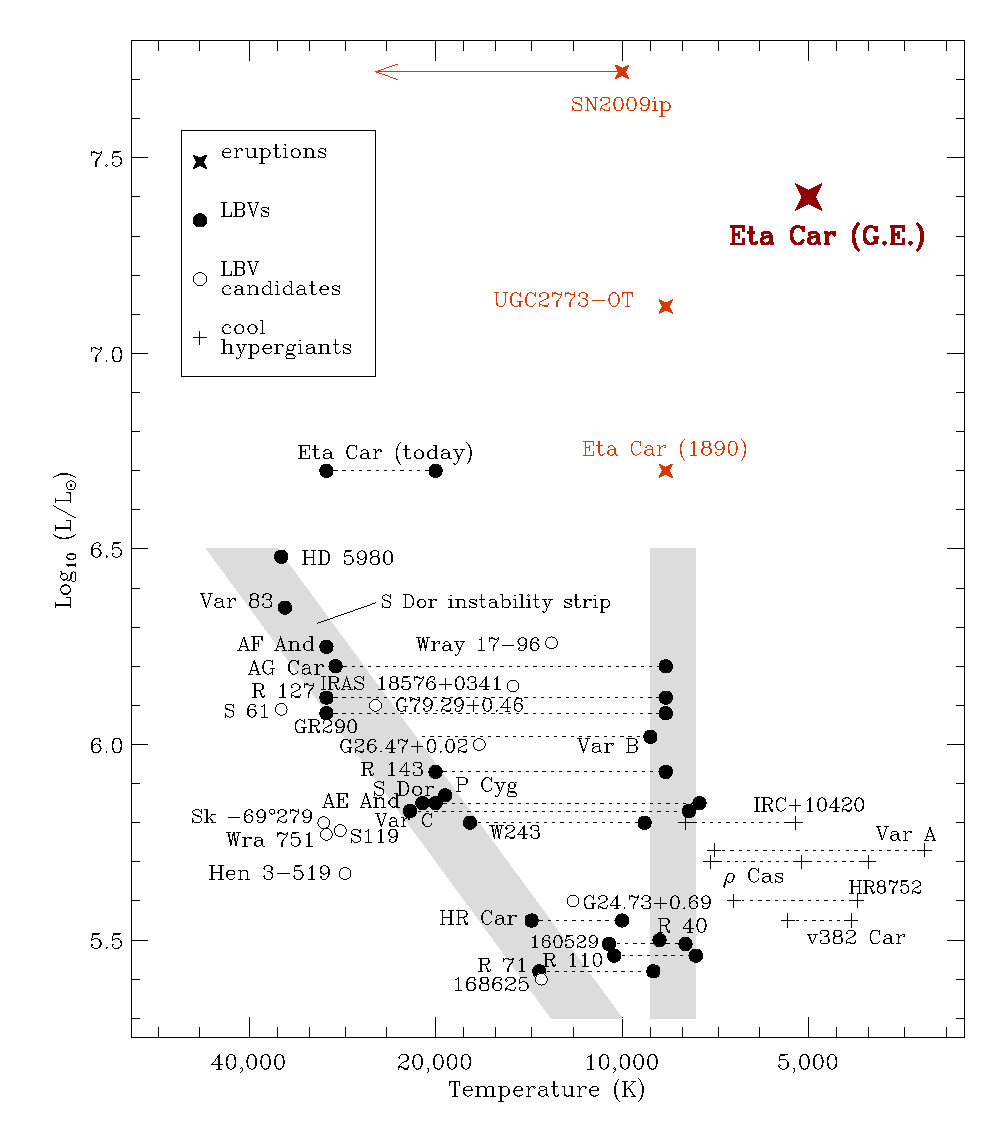
\includegraphics[scale=0.57]{hrdiagram2.jpg}
%\else
%  \ifsuppl
%    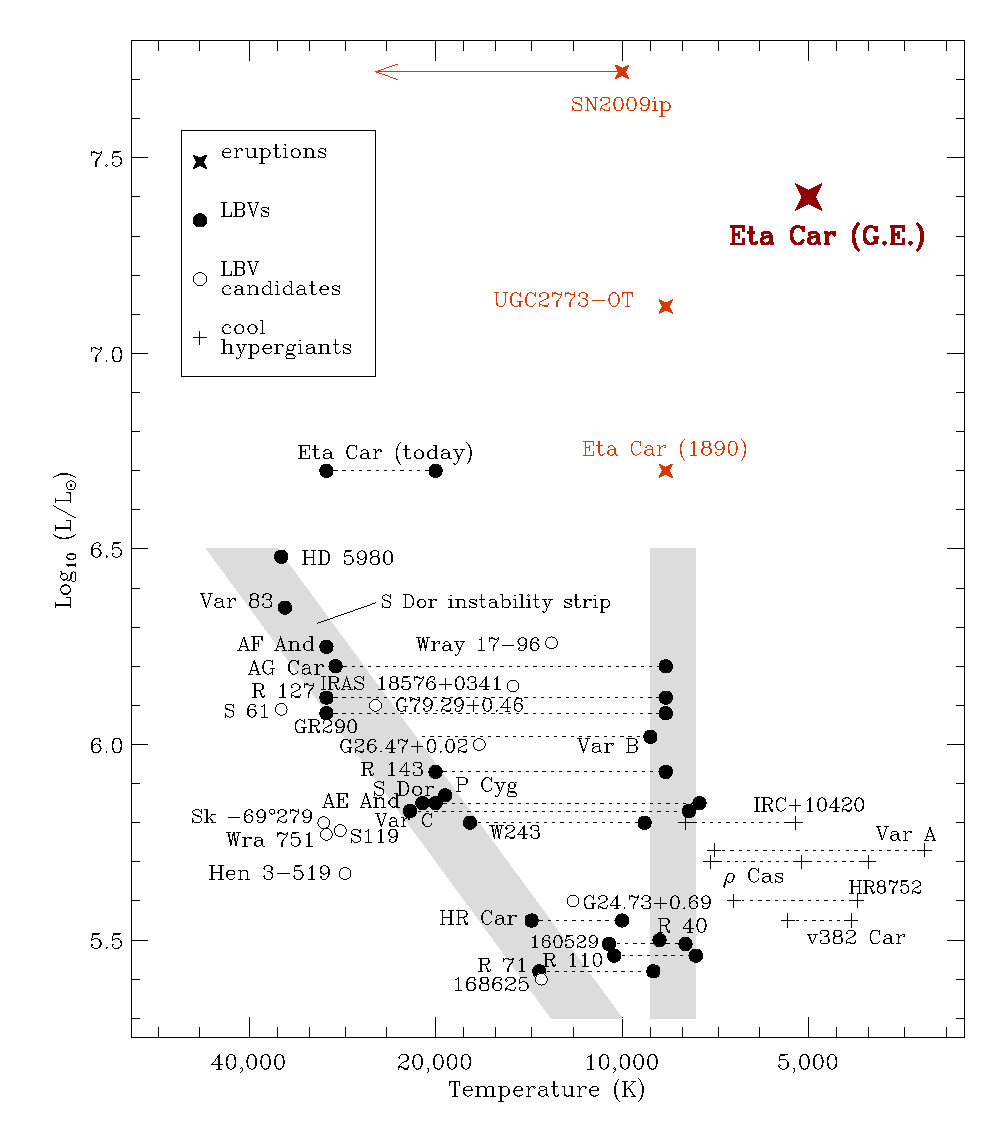
\includegraphics[scale=0.55]{hrdiagram2.jpg}
%  \fi
%\fi
%HR diagram with LBVs and $\eta$~Car.
%Adaptation\cite{Smith04} of an HR diagram showing LBVs, related
%hypergiant stars, and the peak luminosities of LBV-like eruptions. The
%grey bands denote the typical locations of LBVs in quiescence and in S
%Doradus excursions.  Temperatures for the Great Eruption and 1890
%eruption of $\eta$~Car are based on the echo spectra presented here
%and the F-type spectrum of the 1890 event\cite{Walborn77},
%respectively.
%The temperature of 10,000~K for SN~2009ip is based on the observed
%continuum shape, but this is only a lower limit because of the
%possible effects of circumstellar or host galaxy
%reddening\cite{Smith10}.  Because of the presence of \ion{He}{I} lines
%in the spectrum, the true temperature is probably much hotter.
%The 8500~K temperature of UGC2773-OT is indicated by the F-type
%absorption features in its spectrum, and this temperature is
%relatively independent of reddening\cite{Smith10,Foley11}.
%\label{fig:hr}}
%\end{figure}

%\redpen{
%While neither type of LBV outburst is well understood, the traditional
%mechanism for $\eta$~Car-like giant eruptions is an unexplained
%increase in luminosity that drives a denser wind, so that an optically
%thick pseudo-photosphere forms at a layer much larger and cooler than
%the hydrostatic stellar surface\cite{Davidson87}.  As the mass-loss
%rate increases, the effective temperature decreases and the effective
%photosphere of the star moves outward into the wind\cite{Davidson87}.
%This model predicts a minimum effective temperature of $\sim$7000~K
%(an F-type spectrum) since the wind opacity depends on the
%temperature.
%In contrast, S~Dor-type outbursts are suggested to involve an actual
%expansion of the stellar photospheric radius; these events also have
%minimum temperatures in the 7000-9000~K range and exhibit spectra at
%maximum resembling A or F-type supergiants\cite{Humphreys94,Smith04}.
%They evidently occur as a massive star attempts to evolve redward and
%encounter the Humphreys-Davidson Limit\cite{Davidson87}, beyond which
%no stable stars are observed.
%Detailed spectral analysis of LBVs like AG~Car support this
%interpretation by showing that the mass-loss rate does not actually
%increase in an S~Dor event, as would be required to create a
%%pseudo-photosphere in the wind\cite{Groh09}.  Instead, S~Dor-like
%events may be more analogous to a pulsation in which the true
%photosphere expands.
%}

%\clearpage
Surprisingly, our G-type light-echo spectrum of the $\eta$~Car Great
Eruption is inconsistent with expectations of an opaque-wind
model\cite{Davidson87} (see Figure~\ref{fig:hr}). This model also
fails to explain the high 10$^{50}$ erg kinetic energy\cite{Smith03}
and the presence of a fast blast wave at large radii\cite{Smith08}.
Instead, these observations point toward a hydrodynamic explosion 
at least influencing the Great Eruption\cite{Damineli96,Smith03,Smith08}.
%\redpen{Other alternative models
%involving accretion in a binary system have also been
%proposed\cite{Kashi10_ngc300}.}
%The cause that triggered such an explosion and the mass-loss without
%destroying the star is still unknown, but predictions from future
%radiative transfer simulations trying to explain $\eta$~Car and its
%Great Eruption can now be matched to these spectral observations.
%Other alternative models that were proposed, e.g. the ones that use
%mass accretion from the companion star during periapsis passage as a
%trigger for the eruption\cite{Kashi10_ngc300}, can be either verified
%or dismissed.


The first {\it visual} spectroscopic observations of $\eta$~Car around
1870 showed emission lines \cite{LeSueur70a,LeSueur70b}.  A
photographic spectrogram obtained during its Lesser Eruption circa
1890\cite{Walborn77,Humphreys08} resembles an F-type supergiant
blueshifted by $-$200~km~s$^{-1}$, with moderate hydrogen P~Cygni
profiles, which {\it is} as expected in the opaque-wind
model\cite{Davidson87}.  The difference between the 1890 and our
light-echo spectra of the Great Eruption is therefore quite striking,
indicating that two distinct physical processes may have been involved
for two outbursts of the same object.  However, the 1890 event also
produced a mass ejection, the Little Homunculus, with the same axial
symmetry as the Great Eruption\cite{Smith05}, albeit of a much smaller
amount.

LBV giant eruptions are rare, and only have been recorded in our
Galaxy in the last 400 years, the Great Eruption of $\eta$~Car and
P~Cygni's giant eruption in the 17th century.  Because of their
considerable intrinsic brightness just below the luminosity of faint
core-collapse SNe, about two dozen giant eruption candidates,
so-called SN imposters since they have been often mistaken for SNe,
have been found in various extragalactic SN
searches\cite{Goodrich89,Humphreys94,Humphreys99,VanDyk00,Vink09,Kashi10_ngc300}.
%$\eta$~Car's Great Eruption has been considered the prototype of these
%SN imposters or $\eta$~Car analogues, even though it is actually an
%extreme case in terms of radiated energy (10$^{49.3}$ erg), kinetic
%energy ($>$$10^{50}$~erg), and its decade-long duration\cite{Smith11}.
Typically, the hotter SN imposters have steep blue continua, stronger
and broader Balmer lines, and relatively weak absorption, whereas the
cooler ones tend to have redder continua, weaker and narrower Balmer
lines, strong [\ion{Ca}{II}] and \ion{Ca}{II} emission, deeper P~Cygni
absorption features, and in some cases stronger absorption spectra
similar to F-type supergiants\cite{Smith11}.  However, the $\eta$~Car
Great-Eruption light-echo spectrum is quite different.  Its spectral
type is G2-G5, significantly later than all other SN imposters at
peak.  Furthermore, the \ion{Ca}{II} IR triplet lines are only in
absorption.  
%It is difficult to see how strong emission lines could be
%avoided in an opaque wind where the continuum photosphere is
%determined by a change in opacity.
For the extreme mass-loss rates required in $\eta$~Car's Great
Eruption, another process must give rise to the apparent temperature.

%\redpen{\clearpage}
$\eta$~Car's Great Eruption has been considered the prototype of the
extragalactic SN imposters or $\eta$~Car analogues, even though it is
actually an extreme case in terms of radiated energy (10$^{49.3}$
erg), kinetic energy ($>$$10^{50}$~erg), and its decade-long
duration\cite{Smith11}. The spectra of the light echo indicates now
that it is not only extreme, but a different and rather unique object.
It is difficult to see how strong emission lines could be avoided in
an opaque wind where the continuum photosphere is determined by a
change in opacity, and its temperature and broad absorption lines are
more consistent with the opaque cooling photosphere of an explosion.
The cause that triggered such an explosion and the mass-loss without
destroying the star is still unknown, but predictions from future
radiative transfer simulations trying to explain $\eta$~Car and its
Great Eruption can now be matched to these spectral observations.
Other alternative models that were proposed, e.g. the ones that use
mass accretion 
from the companion star during periapsis passage as a
trigger for the eruption\cite{Kashi10_ngc300}, can be either verified
or dismissed. 
\whitepen{\cite{Rest05b,Rest08b,Rest11_leprofile,Smith10,Foley11}}
%$\eta$~Car is a rare example of new types of transients
%in our own backyard, close enough to be studied in detail and for
%which we have information spanning nearly two centuries.
%This allows us to obtain detailed measurements of the mass,
%expansion speed, kinetic energy, and composition of material ejected
%in that event, and compare it to the increasing number of
%extra-galactic transients discovered in the recent time-domain
%wide-field surveys.

%In recent years, time-domain wide-field surveys have discovered in
%increasing numbers explosions or eruptions intermediate in energy and
%luminosity between traditional supernovae and novae. The physical
%mechanisms of this entire class of outbursts is not known. Even though we
%can obtain spectra of these extragalactic outbursts,

%we can obtain spectra of these extragalactic outbursts, but like
%supernovae, we need nearby prototypes to compare to in order to
%measure detailed physical properties.  the best studied object in this
%regard is eta Carinae, which suffered an eruption in the mid 19th
%century that had a luminosity between novae and supernovae, which has
%been assumed to be similar to the class of extragalactic events.
%Because Eta Car is only 2.3 kpc away and because the explosion
%happened only 160 years ago, we have detailed measurements of the
%mass, expansion speed, kinetic energy, and composition of material
%ejected in that event.  Until now, however, we have had no way to
%obtain a spectrum of the eruption itself, since the luminous outburst
%occurred before the invention of the astronomical spectrograph.



%An added complication, of
%course, is that the apparent temperature and other spectral properties
%can evolve with time as an object brightens and fades, as the case of
%SN~2002bu clearly illustrates\cite{Smith11}, and the extreme values may be 
%missed.

%The present spectroscopy of the Eta Car Great Eruption provides new
%constraints and poses more questions for the modeling of these
%enigmatic eruptions.  They will allow us not only to look at the Great
%Eruption from different directions and probe its asymmetry, similarly
%to what has been done for the Cas~A
%SN\cite{Rest11_leprofile,Rest11_casaspec}, but also to obtain a
%spectral time series from each direction by observing at the same
%position during subsequent years.  In addition, in cases where the
%dust filament structure is simple (such as a small isolated dust
%cloud), the shape of the light curve can also be determined.

%\redpen{
%The Great Eruption of $\eta$~Car is one of the most spectacular known
%astronomical events, providing valuable clues for understanding
%massive stars, stellar mass loss, LBVs, and SN imposters.  Yet for a
%century and a half 
%we were missing part of the translation because of
%the technological limitations of the past.
%we were missing critical spectral information about the eruption
%itself, due to the technological limitations of the past.
%The discovery of light echoes from this event gives us a second chance
%to relive one of the legendary and most important events from
%astronomical history, this time with modern equipment.
%The discovery of its light echoes 
%from this event 
%gives us a second chance to relive this important event. The early
%data presented here have already revealed surprises.  Many more will
%come as we continue to watch echoes from the Great Eruption in real
%time, as we follow new echoes from different time periods, and as we
%add spatial information to build a four-dimensional picture of the
%death throes of one of the most interesting objects in the Milky
%Way.}}

